\documentclass[fontsize=10pt]{beamer}
%% Possible paper sizes: a0, a0b, a1, a2, a3, a4.
%% Possible orientations: portrait, landscape
%% Font sizes can be changed using the scale option.
\usepackage[size=custom, width=120, height=90, orientation=landscape, scale=1]{beamerposter}
\usetheme{LLT-poster}
\usecolortheme{ComingClean}
%\usecolortheme{Entrepreneur}
%\usecolortheme{ConspiciousCreep}  %% VERY garish.

%\usepackage[utf8]{inputenc}
\usepackage{libertine}
\usepackage[scaled=1]{inconsolata}
\usepackage{svg}
\usepackage{tabularx}
\usepackage{calc}
\usepackage{makecell}
\usepackage{csquotes}
\usepackage{caption}
\usepackage{mathtools}
\usepackage{arydshln}  % For \hdashline in tables
\usepackage{booktabs}
\usepackage{multirow}

% 1. Load the unicode-math package. This is the modern engine for math fonts.
\usepackage{unicode-math}
\usepackage{mwe}

% Custom operatore and contractions
\newcommand{\ones}{\mathbf 1}
\newcommand{\reals}{{\mbox{\bf R}}}
\newcommand{\integers}{{\mbox{\bf Z}}}
\newcommand{\symm}{{\mbox{\bf S}}}  % symmetric matrices

\newcommand{\nullspace}{{\mathcal N}}
\newcommand{\range}{{\mathcal R}}
\newcommand{\Rank}{\mathop{\bf Rank}}
\newcommand{\Tr}{\mathop{\bf Tr}}
\newcommand{\diag}{\mathop{\bf diag}}
\newcommand{\card}{\mathop{\bf card}}
\newcommand{\rank}{\mathop{\bf rank}}
\newcommand{\conv}{\mathop{\bf conv}}
\newcommand{\prox}{\mathbf{prox}}

\newcommand{\Expect}{\mathop{\bf E{}}}
\newcommand{\Prob}{\mathop{\bf Prob}}
\newcommand{\Co}{{\mathop {\bf Co}}} % convex hull
\newcommand{\dist}{\mathop{\bf dist{}}}
\newcommand{\argmin}{\mathop{\rm argmin}}
\newcommand{\argmax}{\mathop{\rm argmax}}
\newcommand{\epi}{\mathop{\bf epi}} % epigraph
\newcommand{\Vol}{\mathop{\bf vol}}
\newcommand{\dom}{\mathop{\bf dom}} % domain
\newcommand{\intr}{\mathop{\bf int}}
\newcommand{\sign}{\mathop{\bf sign}}

\newcommand{\cf}{{\it cf.}}
\newcommand{\eg}{{\it e.g.}}
\newcommand{\ie}{{\it i.e.}}
\newcommand{\etc}{{\it etc.}}

\newcommand{\norm}[1]{\Vert{#1}\Vert}

% Graphics from the article repo
\graphicspath{{../conf_article/figs/}{../figures/13may_muon_neon/}}

% Define eqspace command (for text mode spacing)
\newcommand{\eqspace}{\par\vspace{0.2em}}

\defineauthorblock{%
  \renewcommand\cellalign{l}
  % We use tabular* spanning slightly less than full width to leave room for margins
  % Then center it to distribute margins equally
  \hspace*{\fill}%
  \begin{tabular*}{\dimexpr\linewidth-4em\relax}{
    @{}
    l
    @{\extracolsep{\fill}}
    l
    l
    l
    l
    l
    l
    @{}
  }
    % --- Column 1: First Author ---
    \makecell{
    \textbf{\Large Alexey Kravatskiy$^{1}$} \\[2ex]
    {\Large kravtskii.aiu@phystech.edu}
    } &

    % --- Column 2: Second Author ---
    \makecell{
    \textbf{\Large Ivan Kozyrev$^{1}$} \\[2ex]
    {\Large kozyrev.in@phystech.edu}
    } &

    % --- Column 3: Third Author ---
    \makecell{
    \textbf{\Large Nikolai Kozlov$^{1}$} \\[2ex]
    {\Large kozlov.na@phystech.edu}
    } &

    % --- Column 4: Fourth Author ---
    \makecell{
    \textbf{\Large Alexander Vinogradov$^{1}$} \\[2ex]
    {\Large vinogradov.am@phystech.edu}
    } &

    % --- Column 5: Fifth Author ---
    \makecell{
    \textbf{\Large Daniil Merkulov$^{1, 2, 3, 4}$} \\[2ex]
    {\Large daniil.merkulov@phystech.edu}
    } &

    % --- Column 6: Sixth Author ---
    \makecell{
    \textbf{\Large Ivan Oseledets$^{5, 2}$} \\[2ex]
    {\Large i.oseledets@skoltech.ru}
    } &

    % --- Column 7: All Institutions ---
    \makecell{
    \Large $^{1}$Moscow Institute of Physics and Technology\\
    \Large $^{2}$Skolkovo Institute of Science and Technology\\
    \Large $^{3}$HSE\; \Large $^{4}$AI4Science\; \Large $^{5}$AIRI
    }
  \end{tabular*}%
  \hspace*{\fill}%
}

\title{The Ky Fan Norms and Beyond: Dual Norms and Combinations for Matrix Optimization}

\begin{document}
\begin{frame}[fragile]
\begin{columns}[T]
\hspace{0.02\textwidth}% Left margin
%%%% First Column
\begin{column}{0.30\textwidth}
% Apply paragraph spacing inside column
\setlength{\parskip}{0.7em}
\setlength{\parindent}{0pt}
\Large

\textbf{\Huge\color{Zen}Introduction}\\[0.3em]

Training large language models requires optimizers more scalable and efficient than Adam/AdamW. The recent Muon~[2] optimizer shows great promise, sometimes doubling AdamW's efficiency, due to its unique design:
\begin{itemize}
  \item \textbf{\color{HazySummerEve}Matrix-Aware Design:} It is constructed specifically for weight matrices, not generic vectors.
  \item \textbf{\color{HazySummerEve}Principled Update Rule:} Muon's update is not merely heuristic. It is derived as the solution to a linear minimization problem constrained by the operator (spectral) norm, giving it a solid mathematical foundation.
\end{itemize}

Muon's success has inspired variants like Dion~[1] algorithm and frameworks of Scion and Gluon~[4]. We build on this work by asking a fundamental question:
\begin{attention}
In deriving Muon's update step, why constrain by the spectral norm? How would alternative norms affect performance and computational cost?
\end{attention}
To investigate this, we first analyze the link between Muon-like algorithms and their defining norms. We then propose \textbf{\color{HazySummerEve}F-Fanions}, a novel family of optimizers derived from exotic, mixed norms. Finally, we present an empirical comparison between Muon and F-Fanions across various numerical experiments.

\vspace{0.5em}
\textbf{\Huge\color{Zen}How Norms Shape the Update Step}\\[0.3em]

Many optimizers are defined by a norm-constrained Linear Minimization Oracle (LMO)~[3], which computes the update $\Delta\mX^t$ based on the gradient (possibly stochastic / with momentum) $\mG^t$:
\begin{equation*}
    \Delta X^t = \mX^{t+1} - \mX^t \in \eta \arg\min_{\norm{\mX} \leq 1} \inner{\mG^t}{\mX}\,.
\end{equation*}
The choice of norm dictates the algorithm. For matrix methods, the update often uses the Singular Value Decomposition (SVD) of the gradient, $\mG^t = \mU \mSigma \mV^\top$.

\centering
% Using 'tabular' now for better width control based on content
\begin{tabular}{clcc}
\toprule
\textbf{Case} & \textbf{Method} & \textbf{Constraining Norm} & \textbf{Update Formula} \\
\midrule
\multirow{3}{*}{\rotatebox[origin=c]{90}{\parbox{1.5cm}{\centering Vec.}}}
& Normalized SGD    & $\ell_2$          & $-\eta g / \norm{g}_2$ \\
& SignSGD           & $\ell_\infty$     & $-\eta\sign(g)$ \\
& Coordinate Descent    & $\ell_1$          & $-\eta e_{\mathrm{argmax}|g_i|}$ \\
\midrule
\multirow{3}{*}{\rotatebox[origin=c]{90}{\parbox{1.5cm}{\centering Mat.}}}
& Normalized SGD    & $\normf{\cdot}$   & $-\eta\mG^t / \normf{\mG^t}$ \\
& Muon     & $\norms{\cdot}$   & $-\eta\mU \mV^\top$ \\
& Dion (no feedback)   & $\norm{\cdot}_{KF-k}^\dag$ & $-\eta\mU_k \mV_k^\top$ \\
\bottomrule
\end{tabular}

\end{column}
\hspace{0.02\textwidth}% Space between columns
%%%% Second Column
\begin{column}{0.30\textwidth}
\setlength{\parskip}{0.7em}
\setlength{\parindent}{0pt}
\Large

We introduce a generalized norm that unifies and interpolates between these methods:
\begin{equation*}
    \norm{\mX}_{\text{gen}} = \left( \alpha \normkfk{\mX} + (1 - \alpha) \normf{\mX} \right)^\dag\,.
\end{equation*}

This defines the \textbf{\color{HazySummerEve}F-Fanions}, a new family of optimizers parameterized by $\alpha \in [0, 1]$ and $k$, with the update rule:
\begin{equation*}
    \Delta \mX^t = \eta \alpha \mU_k \mV_k^\top + \eta(1 - \alpha) \frac{\mG^t}{\normf{\mG^t}}\,.
\end{equation*}

This framework recovers existing algorithms as special cases:
\begin{itemize}
    \item \textbf{\color{HazySummerEve}Normalized SGD:} $\alpha = 0$.
    \item \textbf{\color{HazySummerEve}Dion} (no feedback): $\alpha = 1$, $k < \min\{m, n\}$.
    \item \textbf{\color{HazySummerEve}Muon:} $\alpha = 1$, $k = \min\{m, n\}$.
\end{itemize}
We also identify and analyze \textbf{\color{HazySummerEve}F-Neon}, a computationally efficient member of this family where $k=1$.

\vspace{0.5em}
\textbf{\Huge\color{Zen}Efficiently Computing the Update}\\[0.3em]

Computing the F-Fanion update is efficient at the extremes of the rank parameter $k$. We propose using the GPU-friendly \textbf{\color{HazySummerEve}Thick-Restarted Lanczos (TRLan)} method in two distinct ways:
\begin{itemize}
    \item \textbf{\color{HazySummerEve}For small $k$ (e.g., F-Neon):} TRLan is used directly to find the few leading singular vectors.
    \item \textbf{\color{HazySummerEve}For large $k$ (e.g., Muon):} TRLan is used to compute trailing singular values, they are substracted from a full-rank term, obtained through Newton-Shulz iterations.
\end{itemize}

The table below demonstrates the speed of the direct approach for finding $k$ leading singular vectors, from a $5000 \times 5000$ matrix. 

{
\centering
\begin{tabular}{lccc}
\toprule
\textbf{Method} & \textbf{k=1} & \textbf{k=10} & \textbf{k=100} \\
\midrule
TRLan (our choice) & 0.18s & 0.47s & 1.96s \\
Randomized SVD (RSVD)       & 1.15s          & 19.4s          & 170.0s \\
Power Iterations            & 7.70s          & ---            & --- \\
\bottomrule
\end{tabular}
\par
\vspace{0.5em}
}

TRLan's dramatic speed advantage in this direct computation makes low-rank F-Fanions, like F-Neon, highly efficient.

\vspace{0.5em}
\textbf{\Huge\color{Zen}Modded NanoGPT Speedrun}\\[0.3em]

We benchmarked our method against Muon on the \texttt{modded\_nanogpt\_2024} speedrun, a time-constrained training challenge. Below are the results after 1750 steps, 

{
\centering
\begin{tabular}{lccc}
\toprule
\textbf{Method} & \textbf{LR} & \textbf{Momentum} & \textbf{Final Loss} \\
\midrule
Muon (Baseline) & 0.05 & 0.95 & 3.279 (Pass) \\
F-Muon ($\alpha=0.5$) & 0.07 & 0.95 & 3.281 (Near Miss) \\
\bottomrule
\end{tabular}
\par
}

\end{column}
\hspace{0.02\textwidth}% Space between columns

%%%% Third column
\begin{column}{0.30\textwidth}
\setlength{\parskip}{0.7em}
\setlength{\parindent}{0pt}
\Large

\textbf{\Huge\color{Zen}CIFAR-10 Airbench Experiments}\\[0.3em]

We evaluate F-Muon against Muon by training a Convolutional Neural Network (CNN) on the CIFAR-10 Airbench. All results are averaged over multiple runs after 8 epochs.

\begin{columns}[T,totalwidth=\textwidth]
      \begin{column}{0.48\textwidth}
        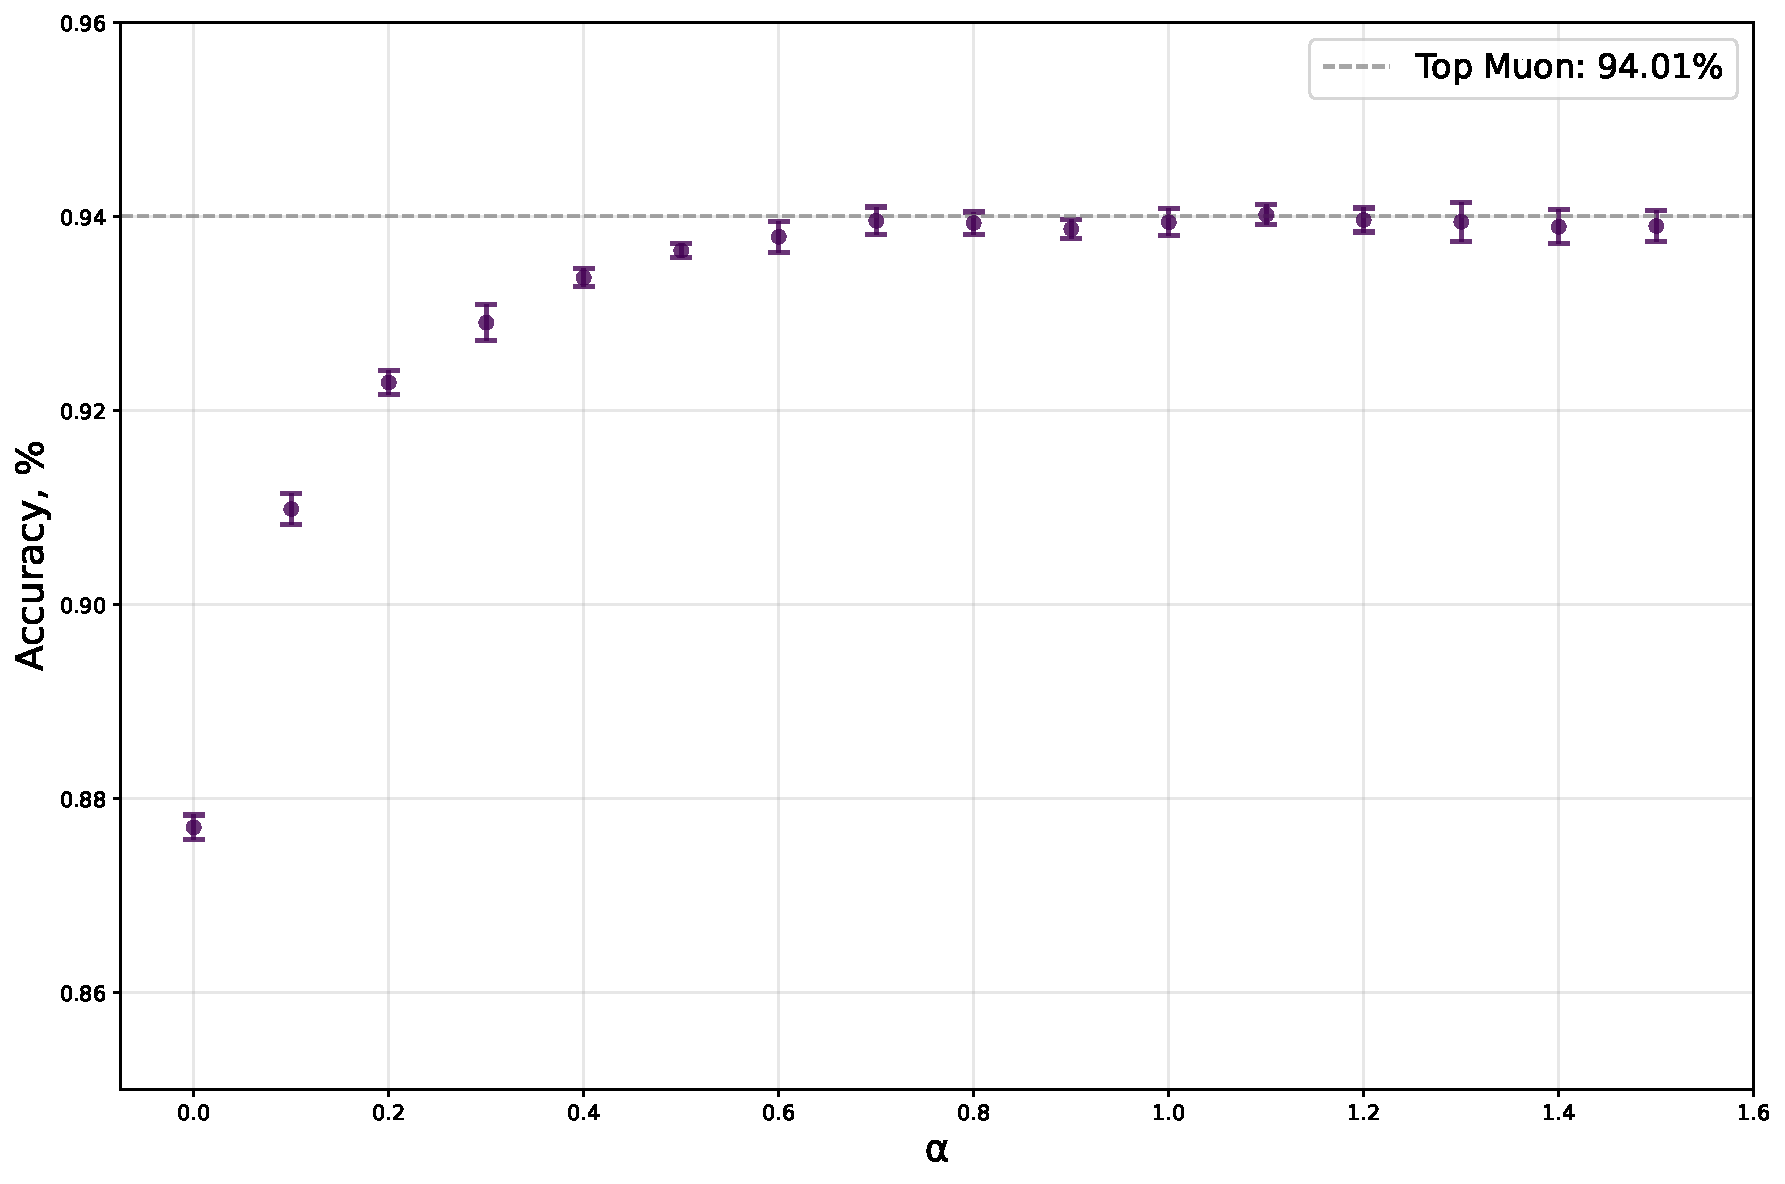
\includegraphics[width=\linewidth]{muon_tuned_diff_alpha.pdf}

        {\centering With parameters from tuned version of Muon\par}
      \end{column}
      \begin{column}{0.48\textwidth}
        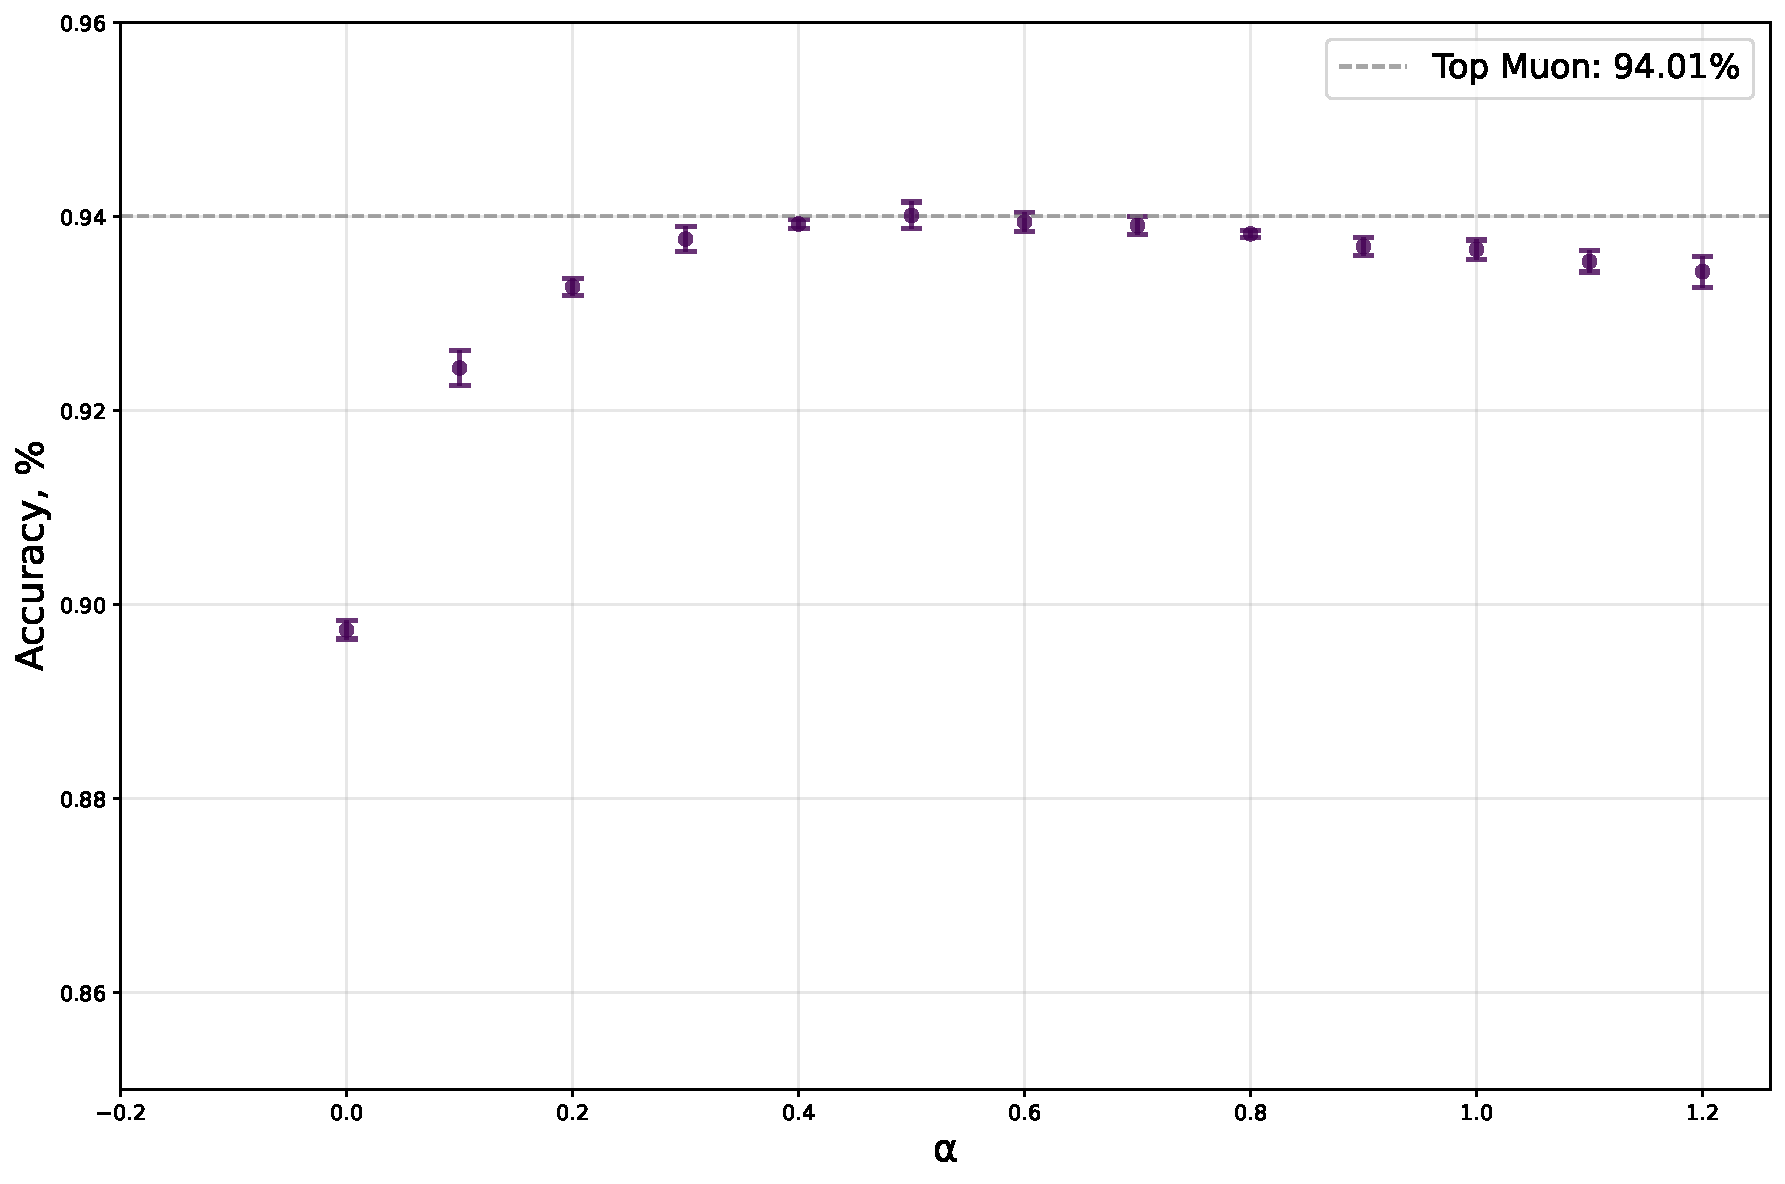
\includegraphics[width=\linewidth]{fmuon_tuned_diff_alpha.pdf}

        {\centering With parameters tuned for F-Muon, $\alpha = 0.5$\par}
      \end{column}
    \end{columns}\vspace{1em}

\begin{columns}[T,totalwidth=\textwidth]
  \begin{column}{0.47\textwidth}
    \setlength{\parskip}{0.7em}
\setlength{\parindent}{0pt}
\Large
    We can see that Properly tuned F-Muon can perform on par with Muon, achieving the same 94\% accuracy. 
    
    Another Interesting observation here is that tuned F-Muon has much larger trust region then Muon, and thus makes larger step sizes (figure to the right).
  \end{column}
  \begin{column}{0.49\textwidth}
    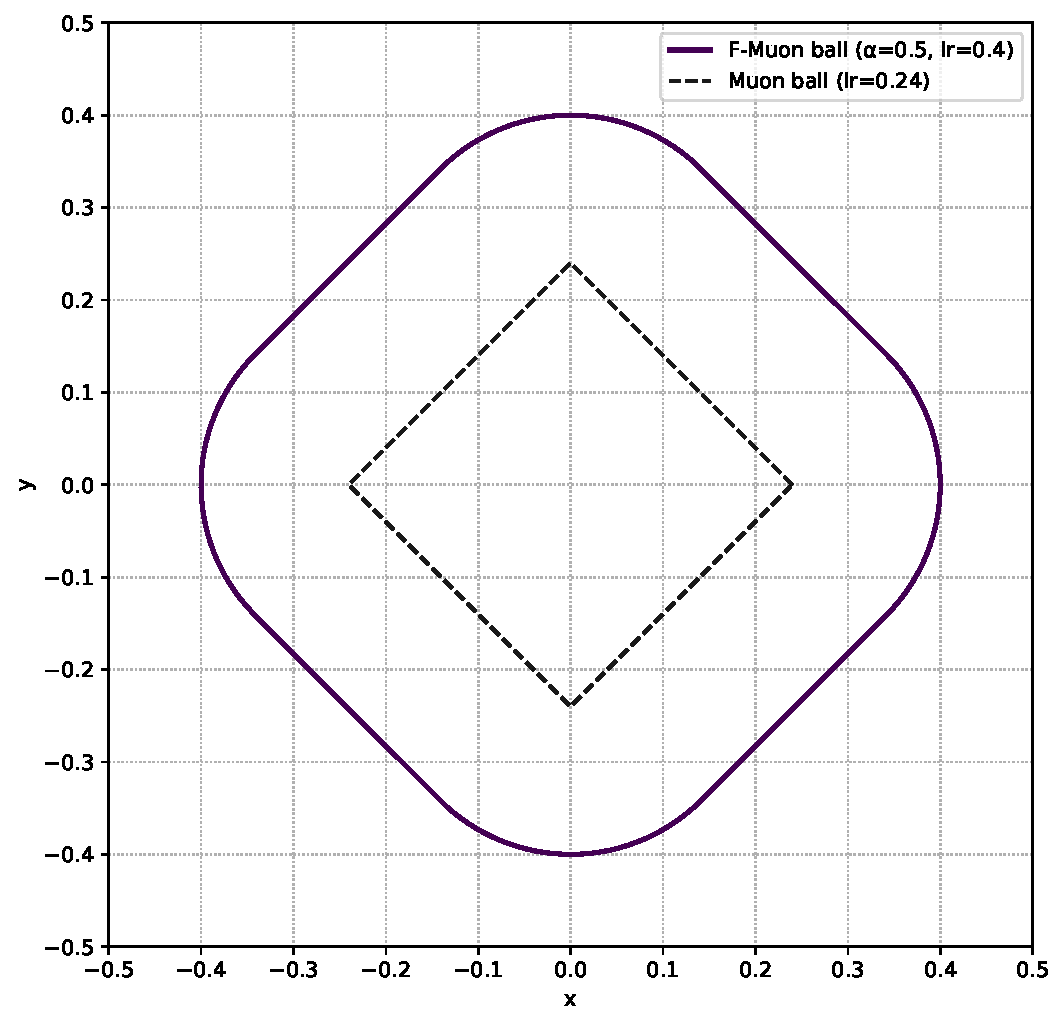
\includegraphics[width=\linewidth]{fstardual_cifar.pdf}
    \centering
  \end{column}
\end{columns}

\vspace{0.5em}
\textbf{\Huge\color{Zen}Conclusion \& Outlook}\\[0.6em]

\begin{itemize}
    \item We introduced the \textbf{\color{HazySummerEve}F-Fanion framework}, unifying LMO-based optimizers like Muon and Dion via mixed norms. 

    \item The choice of norm is a flexible design parameter, not a fixed rule. Our results show alternatives to the spectral norm can be equally effective.

    \item This work opens the core question of how to theoretically guide norm selection. Future work could also explore adapting the norm (via $\alpha$ and $k$) dynamically during training.
\end{itemize}

\vspace{0.5em}
\textbf{\Huge\color{Zen}Key References}\\[0.6em]

\begin{itemize}
   \large
    \setlength{\itemsep}{0pt} % Remove spacing between items
    \item[{[1]}] Ahn, K. \& Xu, B. *Dion*. arXiv:2504.05295, 2025.
    \item[{[2]}] Bernstein, J. *Deriving muon*. 2025. URL: jeremybernste.in/writing/deriving-muon
    \item[{[3]}] Bernstein, J. \& Newhouse, L. *Old optimizer, new norm*. arXiv:2409.20325, 2024.
    \item[{[4]}] Riabinin, A. et al. *Gluon: Making muon \& scion great again!* arXiv:2505.13416, 2025.
\end{itemize}

\end{column}
\hspace*{0.02\textwidth}% Right margin (using \hspace* to prevent it from being dropped)
\end{columns}

\end{frame}
\end{document}